\section{Analisis dan Perancangan Sistem}
\label{sec:analisisperancangansistem}

Analisis sistem dilakukan untuk memahami alur kerja internal Bapenda serta kebutuhan fungsional dari setiap modul yang akan dikembangkan. Hasil analisis ini kemudian menjadi dasar dalam perancangan arsitektur sistem, struktur \emph{ViewModel}, dan desain antarmuka pengguna.

\subsection{Analisis Kebutuhan Fungsional}
Berdasarkan diskusi dan analisis, diidentifikasi kebutuhan fungsional yang menjadi dasar pengembangan MonPD Reborn. Detailnya disajikan dalam Tabel \ref{tab:kebutuhan_fungsional}.

\renewcommand{\arraystretch}{1.5}

% Menggunakan kolom p{} agar teks membungkus (wrap) dengan benar di kertas A5
\begin{longtable}{|c|p{2cm}|p{2cm}|p{4cm}|}
\caption{Analisis Kebutuhan Fungsional MonPD Reborn}
\label{tab:kebutuhan_fungsional} \\
\hline
\textbf{No} & \textbf{Menu Utama} & \textbf{Sub-menu} & \textbf{Deskripsi Kebutuhan} \\ \hline
\endfirsthead

\hline
\textbf{No} & \textbf{Menu Utama} & \textbf{Sub-menu} & \textbf{Deskripsi Kebutuhan} \\ \hline
\endhead

\hline
\endfoot

\hline
\endlastfoot

1 & \multirow{8}{2cm}{Objek Pajak} & Series Pendapatan & Menampilkan data historis pendapatan daerah dalam bentuk \emph{series}. \\ \cline{1-1} \cline{3-4}
2 &  & Pengedokan Pajak & Modul untuk memantau aktivitas pendataan potensi pajak di lapangan. \\ \cline{1-1} \cline{3-4}
3 &  & Pemeriksaan Pajak & Menampilkan rekapitulasi dan detail hasil pemeriksaan objek pajak. \\ \cline{1-1} \cline{3-4}
4 &  & Alat Rekam \emph{Online} & Memonitor data dari alat rekam transaksi (\emph{tapping box}). \\ \cline{1-1} \cline{3-4}
5 &  & Realisasi Kontrol & Menyajikan perbandingan antara target dan realisasi secara detail. \\ \cline{1-1} \cline{3-4}
6 &  & Data OP & Akses untuk melihat dan mengelola data \emph{master} Objek Pajak. \\ \cline{1-1} \cline{3-4}
7 &  & Monitoring Capaian & \emph{Dashboard} untuk memantau progres pencapaian target. \\ \cline{1-1} \cline{3-4}
8 &  & Monitoring Wilayah & Membandingkan capaian pendapatan antar wilayah kerja (UPTB). \\ \hline

9 & \multirow{4}{2cm}{Pengawasan Reklame} & Reklame \emph{Summary} & Menampilkan ringkasan data agregat jumlah reklame dan potensi pendapatan. \\ \cline{1-1} \cline{3-4}
10 &  & Kontrol Reklame & Modul melakukan kontrol dan validasi terhadap data reklame. \\ \cline{1-1} \cline{3-4}
11 &  & Reklame Liar & Mencatat laporan mengenai reklame yang tidak berizin. \\ \cline{1-1} \cline{3-4}
12 &  & Pendataan Reklame & Antarmuka untuk proses pendataan titik reklame baru. \\ \hline

13 & \multirow{4}{2cm}{Wajib Pajak} & Aktivitas Penghimbauan & Mencatat dan memonitor kegiatan penghimbauan kepada WP. \\ \cline{1-1} \cline{3-4}
14 &  & Aktivitas Peneguran & Melacak pengiriman surat teguran kepada WP yang menunggak. \\ \cline{1-1} \cline{3-4}
15 &  & Aktivitas Penagihan & Memantau siklus penagihan aktif. \\ \cline{1-1} \cline{3-4}
16 &  & Data WP & Akses terpusat profil dan riwayat data Wajib Pajak. \\ \hline

17 & \multirow{2}{2cm}{Laporan Strategis} & Evaluasi Target & Laporan perbandingan target dengan realisasi periode tertentu. \\ \cline{1-1} \cline{3-4}
18 &  & Analisis Tren & Menyajikan analisis kenaikan atau penurunan pendapatan. \\ \hline
\end{longtable}


\subsection{Perancangan Arsitektur Sistem}
Sistem ini dibangun menggunakan arsitektur \emph{Model View Controller} (MVC) yang disediakan oleh \emph{framework} ASP.NET Core dengan bahasa pemrograman C\#. Pola arsitektur ini dipilih karena kemampuannya memisahkan antara logika bisnis, data, dan presentasi, sehingga menghasilkan struktur kode yang rapi, modular, dan mudah dikelola.
\begin{itemize}
    \item \textbf{\emph{Model}}: \\
    Terdiri dari serangkaian kelas \emph{ViewModel} (VM) yang dirancang khusus untuk setiap halaman. \emph{ViewModel} ini berfungsi sebagai ``cetakan'' data yang akan dikirim ke antarmuka, menggabungkan data dari berbagai sumber dan mengolahnya sesuai kebutuhan tampilan. Di dalam \emph{ViewModel}, terdapat juga kelas \emph{Method} yang berisi logika untuk mengambil dan memanipulasi data (baik data \emph{dummy} maupun dari basis data). \\
    Salah satu keputusan desain arsitektur yang penting adalah menempatkan sebagian besar logika bisnis di dalam \emph{Method} pada setiap \emph{ViewModel}. Dengan pendekatan ini, \emph{Controller} hanya bertugas sebagai penerus permintaan. Contohnya, pada \emph{ViewModel} \texttt{ReklameLiarVM}, terdapat lebih dari 5 \emph{class} yang berbeda (\texttt{Index}, \texttt{Show}, \texttt{Detail}, \texttt{RekapBulanan}, \texttt{DetailData}) untuk melayani setiap kebutuhan data yang spesifik, mulai dari data rekap bulanan hingga data detail untuk \emph{modal pop-up}.
    \item \textbf{\emph{View}}: \\
    Terdiri dari file-file \texttt{.cshtml} (\emph{Razor}) yang bertanggung jawab untuk menampilkan antarmuka pengguna. Halaman \emph{View} menerima data dari \emph{Controller} melalui objek \emph{ViewModel} dan menampilkannya dalam bentuk \emph{dashboard}, tabel, dan formulir. Sebagian besar tampilan tabel interaktif diimplementasikan menggunakan komponen dari \texttt{DevExtreme}.
    \item \textbf{\emph{Controller}}: \\
    Berperan sebagai jembatan antara \emph{Model} dan \emph{View}. \emph{Controller} menerima permintaan HTTP dari pengguna (misalnya, saat filter diterapkan), memanggil \emph{Method} yang sesuai di dalam \emph{ViewModel} untuk mendapatkan data, lalu mengirimkan data tersebut ke \emph{View} yang relevan untuk ditampilkan kepada pengguna.
\end{itemize}

\subsection{Perancangan \emph{Database}}
Aplikasi ini berinteraksi dengan basis data yang sudah ada di \emph{server database} Bapenda. Koneksi dan manipulasi data dari aplikasi ke basis data ditangani menggunakan \emph{Entity Framework Core}, dengan kelas \texttt{DBContext} yang berfungsi sebagai gerbang utama. Data yang digunakan selama pengembangan bersifat data riil, sehingga struktur \emph{ViewModel} dan logika aplikasi dirancang untuk dapat terhubung langsung dengan tabel-tabel utama seperti \texttt{TPemeriksaan}, \texttt{DbMonResto}, \texttt{DbMonParkir}, dan lainnya, yang merepresentasikan data riil di \emph{server database} Bapenda.

\subsection{Perancangan Antarmuka (UI/UX)}

Perancangan antarmuka pada sistem MonPD Reborn dilakukan dengan mengedepankan prinsip \emph{Information Hierarchy} dan efisiensi operasional. Mengingat sistem ini digunakan untuk memonitor data perpajakan yang sangat besar, setiap halaman dirancang untuk meminimalkan beban kognitif pengguna melalui penempatan elemen yang strategis. Berikut adalah rincian rancangan tata letak dan fungsionalitas pada setiap bagian utama sistem:

\begin{itemize}
    \item Rancangan Pusat Komando (\emph{Command Center}) \\
    Tampilan utama atau \emph{dashboard} dirancang menggunakan tata letak berbasis kartu (\emph{card-based layout}) untuk memberikan ringkasan performa seluruh jenis pajak dalam satu layar tunggal sebagaimana ditunjukkan pada Gambar \ref{fig:wireframe-dashboard-utama-monpd}.
    \begin{figure}[H]
        \centering
        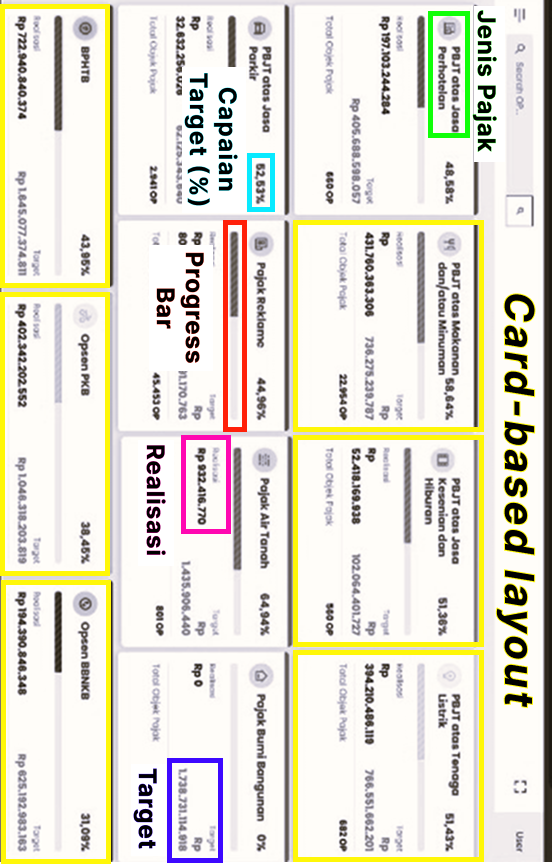
\includegraphics[width=0.9\textwidth]{gambar/wireframe-dashboard-utama-monpd.png}
        \caption{\emph{Wireframe Dashboard} Utama MonPD Reborn}
        \label{fig:wireframe-dashboard-utama-monpd}
    \end{figure}
    \begin{itemize}
        \item \textbf{Fitur Utama:}
            \begin{itemize}
                \item \textbf{Jenis Pajak:} Menampilkan label jenis pajak (eg: Perhotelan, Restoran, Parkir) untuk memudahkan klasifikasi data.
                \item \textbf{Metrik Capaian:} Persentase angka realisasi terhadap target yang dihitung secara \emph{real-time} untuk memberikan indikator kinerja utama.
                \item \textbf{Indikator Visual:} \emph{Progress bar} yang memberikan representasi visual dari persentase capaian memudahkan pemindaian cepat.
                \item \textbf{Komparasi Finansial:} Penyajian nominal Realisasi (pendapatan yang sudah masuk) dan Target (sasaran tahunan).
            \end{itemize}

        \item \textbf{Analisis Penempatan:}
            \begin{itemize}
                \item \textbf{Hierarki Informasi Kartu:} Penggunaan \emph{card-based layout} berfungsi untuk melakukan enkapsulasi data. Setiap jenis pajak memiliki kontainer visualnya sendiri, mencegah terjadinya tumpang tindih informasi antar sektor pajak yang berbeda.
                \item \textbf{Strategi \emph{Visual Cues}:} Penempatan Metrik Capaian dan \emph{Progress Bar} diletakkan di bagian atas kartu. Hal ini didasarkan pada pola baca pengguna yang cenderung memprioritaskan kesimpulan performa (pencapaian) sebelum melihat rincian nominal pendukungnya.
                \item \textbf{Penyandingan Vertikal:} Nominal Realisasi diletakkan di sebelah nominal Target. Penempatan ini dirancang untuk mempermudah perbandingan visual langsung antar dua angka finansial yang berkaitan, sehingga pengguna dapat langsung mengetahui selisih antara pencapaian saat ini dengan target akhir.
            \end{itemize}
    \end{itemize}

    \item Rancangan Struktur Modul Analitik \\
    Setiap modul analitik (misalnya Monitoring Wilayah) menggunakan \emph{standardized template} tiga lapis yang konsisten untuk menciptakan alur kerja yang intuitif bagi pengguna sebagaimana ditunjukkan pada Gambar \ref{fig:wireframe-dashboard-menu-monpd}.
    \begin{figure}[H]
        \centering
        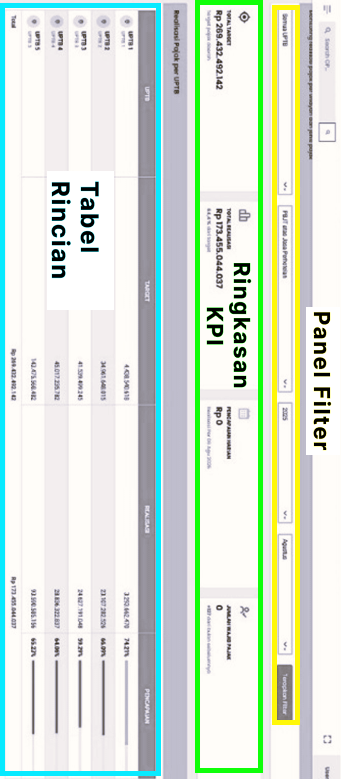
\includegraphics[width=0.65\textwidth]{gambar/wireframe-dashboard-menu-monpd.png}
        \caption{\emph{Wireframe Dashboard} Menu MonPD Reborn}
        \label{fig:wireframe-dashboard-menu-monpd}
    \end{figure}
    \begin{itemize}
        \item \textbf{Fitur Utama:}
            \begin{itemize}
                \item \textbf{Panel Filter:} Terdiri dari komponen \emph{dropdown} untuk pemilihan wilayah (UPTB), jenis pajak, tahun, dan bulan, serta tombol eksekusi "Terapkan Filter".
                \item \textbf{Ringkasan KPI:} Menampilkan kartu-kartu metrik utama (\emph{Key Performance Indicators}) seperti Total Target, Total Realisasi, Pencapaian Harian, dan Jumlah Wajib Pajak (ini bukan standar, karena KPI tiap menu memiliki komponen berbeda).
                \item \textbf{Tabel Rincian:} Menyajikan data rincian per baris yang dilengkapi dengan kolom Target, Realisasi, serta visualisasi \emph{progress bar} untuk setiap baris data.
            \end{itemize}

        \item \textbf{Analisis Penempatan:}
            \begin{itemize}
                \item \textbf{Strategi \emph{Top-Down Workflow}:} Penempatan \textbf{Panel Filter} di posisi teratas berfungsi sebagai gerbang utama operasional. Hal ini menerapkan prinsip \emph{Progressive Disclosure}, di mana sistem membatasi pemuatan data secara masif di awal untuk menjaga performa (\emph{load time}), dan baru akan menarik data spesifik setelah pengguna menentukan parameter pilihannya.
                \item \textbf{Hierarki Kognitif \emph{Summary-to-Detail}:} \textbf{Ringkasan KPI} diletakkan di bagian tengah sebagai jembatan informasi. Secara psikologis, pengguna memerlukan konklusi cepat (angka agregat) segera setelah menerapkan filter, sebelum akhirnya melakukan eksplorasi mendalam pada data baris demi baris di bagian bawah.
                \item \textbf{Optimalisasi Ruang Kerja Tabel:} \textbf{Tabel Rincian} diletakkan sebagai elemen paling luas di bagian bawah. Penempatan ini memberikan ruang visual yang maksimal bagi komponen \emph{DevExtreme DataGrid} untuk menampilkan banyak kolom data secara komprehensif tanpa terasa sesak, sehingga memudahkan proses analisis rincian transaksi oleh pegawai Bapenda.
            \end{itemize}
    \end{itemize}

    \item Rancangan Interaktivitas Data (\emph{DataGrid}) \\
    Komponen \emph{DataGrid} dirancang sebagai pusat eksplorasi data yang memungkinkan pengguna melakukan manipulasi informasi secara mandiri tanpa perlu bergantung pada proses pemuatan ulang halaman (\emph{refresh}) sebagaimana ditunjukkan pada Gambar \ref{fig:wireframe-datagrid}.
    \begin{figure}[H]
        \centering
        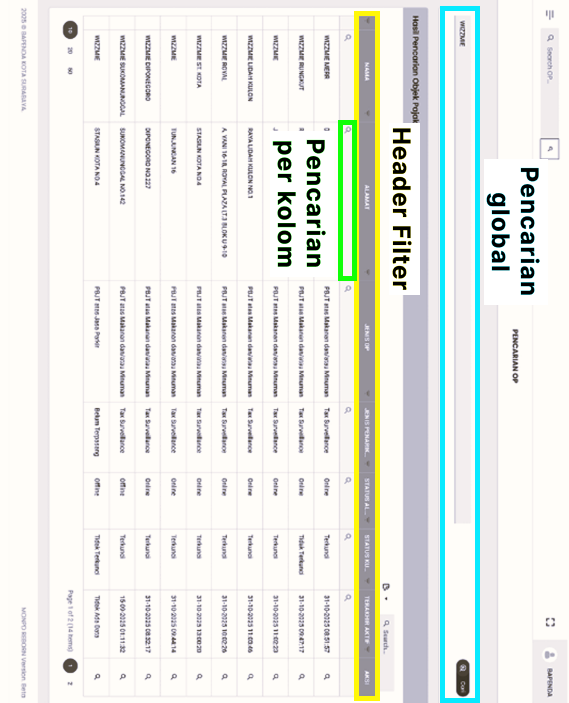
\includegraphics[width=0.96\textwidth]{gambar/wireframe-datagrid.png}
        \caption{\emph{Wireframe DataGrid}}
        \label{fig:wireframe-datagrid}
    \end{figure}
    \begin{itemize}
        \item \textbf{Fitur Utama:}
            \begin{itemize}
                \item \textbf{Pencarian Global:} Fitur pencarian tingkat tinggi di pojok kanan atas yang memungkinkan pengguna mencari kata kunci tertentu di seluruh kolom tabel secara simultan.
                \item \textbf{\emph{Header Filter} dan \emph{Sorting}:} Setiap judul kolom (\emph{Nama, Alamat, Jenis OP}, dll.) dilengkapi dengan fungsi pengurutan (\emph{sorting}) naik atau turun serta filter nilai unik (\emph{header filter}) untuk mempersempit kategori data.
                \item \textbf{Pencarian Per Kolom:} Baris filter (\emph{filter row}) yang terletak tepat di bawah \emph{header}. Fitur ini memungkinkan pengguna melakukan penyaringan data secara spesifik pada kolom tertentu, seperti mencari nama Wajib Pajak tanpa mencampuradukkan dengan data alamat.
                \item \textbf{Navigasi Halaman:} Terletak di bagian bawah kiri, fitur ini membatasi jumlah data yang tampil per layar untuk menjaga performa \emph{rendering} pada sisi \emph{client}.
            \end{itemize}

        \item \textbf{Analisis Penempatan:}
            \begin{itemize}
                \item \textbf{Konvensi Standar Pencarian Global:} Penempatan \textbf{Pencarian Global} di bagian atas kanan mengikuti standar \emph{User Interface} yang umum, memudahkan pengguna baru untuk langsung mengenali titik awal pencarian informasi secara cepat.
                \item \textbf{Kedekatan Kontekstual:} Penempatan \textbf{Pencarian Per Kolom} dan \textbf{\emph{Header Filter}} yang melekat langsung pada baris judul kolom bertujuan untuk efisiensi kognitif. Pengguna tidak perlu memindahkan fokus pandangan terlalu jauh dari data yang sedang diamati untuk melakukan penyaringan informasi yang lebih granular.
                \item \textbf{Kontrol Presisi Data:} Dengan adanya baris filter khusus per kolom, beban kerja sistem menjadi lebih efisien karena kueri yang dikirim ke server (\emph{server-side filtering}) menjadi lebih spesifik, mengurangi potensi beban \emph{payload} data yang tidak relevan.
                \item \textbf{Manajemen Beban Visual:} \textbf{\emph{Pagination}} diletakkan di bagian akhir alur konsumsi data (bawah). Hal ini memastikan pengguna hanya fokus pada subset data tertentu pada satu waktu, yang secara teknis mendukung tujuan utama \emph{MonPD Reborn} dalam mereduksi waktu muat data secara signifikan.
            \end{itemize}
    \end{itemize}

    \item Rancangan \emph{Drill-down} dan \emph{Pop-up} Detail \\
    Untuk memberikan akses informasi yang lebih mendalam tanpa mengganggu alur kerja pengguna, sistem menyediakan fitur \emph{drill-down} yang memungkinkan rincian data tampil secara transisi.    
    \begin{itemize}
        \item \textbf{Fitur:} Jendela \emph{modal pop-up} yang menampilkan rincian transaksi individu secara spesifik.
        \item \textbf{Analisis Penempatan:} Penggunaan jendela \emph{modal} di atas halaman utama bertujuan untuk menjaga \emph{context-awareness} pengguna. Dengan tetap menampilkan latar belakang halaman rekapitulasi yang sedikit meredup, pengguna akan tetap ingat pada parameter filter atau kategori data awal yang sedang mereka amati saat melihat detail transaksi.
    \end{itemize}

    \item Rancangan Visualisasi Geospasial \\
    Penyajian data berbasis lokasi dirancang untuk memberikan pemahaman spasial terhadap sebaran objek pajak di wilayah Kota Surabaya sebagaimana ditunjukkan pada Gambar \ref{fig:wireframe-geospasial}.
    \begin{figure}[H]
        \centering
        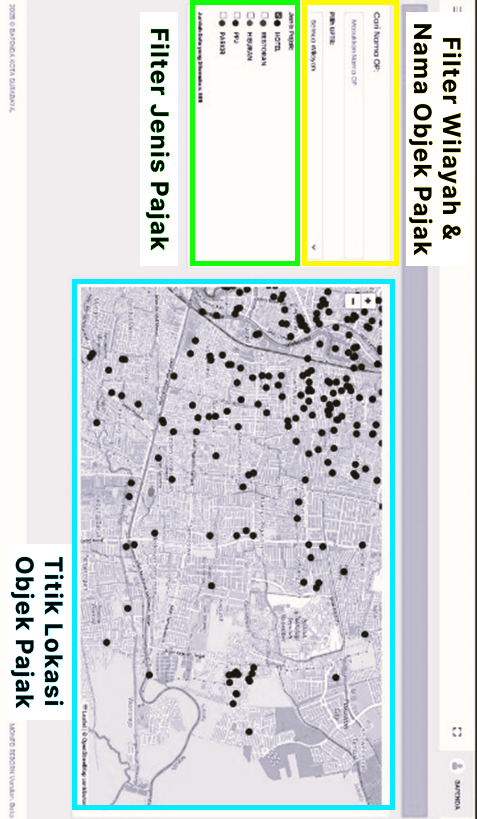
\includegraphics[width=0.73\textwidth]{gambar/wireframe-geospasial.png}
        \caption{Wireframe Visualisasi Geospasial}
        \label{fig:wireframe-geospasial}
    \end{figure}
    \begin{itemize}
        \item \textbf{Fitur Utama:}
            \begin{itemize}
                \item \textbf{Kontrol Pencarian dan Wilayah:} Terdiri dari kolom input "Cari Nama OP" untuk pencarian spesifik entitas pajak dan \emph{dropdown} "Pilih UPTB" untuk membatasi cakupan wilayah kerja administratif.
                \item \textbf{Filter Kategori:} Menyediakan daftar pilihan \emph{checkbox} jenis pajak (Hotel, Restoran, Hiburan, PPJ, Parkir) yang memungkinkan pengguna melakukan \emph{overlaying} data dari berbagai sektor pajak secara bersamaan.
                \item \textbf{Kanvas Pemetaan:} Area peta interaktif yang menampilkan \emph{plotting} titik-titik koordinat objek pajak secara \emph{real-time} berdasarkan parameter filter yang diterapkan.
            \end{itemize}

        \item \textbf{Analisis Penempatan:}
            \begin{itemize}
                \item \textbf{Aksesibilitas Kontrol:} Penempatan panel filter di sisi atas dan samping kiri mengikuti pola pandangan manusia yang memulai pemindaian dari pojok kiri atas. Hal ini memastikan pengguna dapat dengan cepat memodifikasi parameter data sebelum beralih ke analisis visual pada peta.
                \item \textbf{Fokus Analisis Spasial:} Area peta diletakkan sebagai elemen pusat dengan dimensi paling luas. Penempatan ini bertujuan untuk meminimalisir distraksi visual lain, sehingga tim lapangan dapat memfokuskan perhatian sepenuhnya pada kepadatan (\emph{clustering}) titik objek pajak.
                \item \textbf{Efisiensi Perencanaan Rute:} Integrasi antara filter wilayah (UPTB) dan titik lokasi dirancang untuk mempermudah operasional pengawasan di lapangan. Dengan melihat kepadatan titik pada satu wilayah UPTB tertentu, tim pengawas dapat merencanakan rute inspeksi yang paling efisien berdasarkan jarak antar objek pajak, yang pada akhirnya meningkatkan produktivitas kerja.
            \end{itemize}
    \end{itemize}


    \item Rancangan Komparasi Realisasi Pajak \\
    Penyajian data rekapitulasi kinerja dirancang untuk memberikan gambaran cepat mengenai efektivitas pemungutan pajak melalui perbandingan rencana strategis (\emph{target}) terhadap pencapaian aktual (\emph{realisasi}) sebagaimana ditunjukkan pada Gambar \ref{fig:wireframe-realisasi-pajak}.
    \begin{figure}[H]
        \centering
        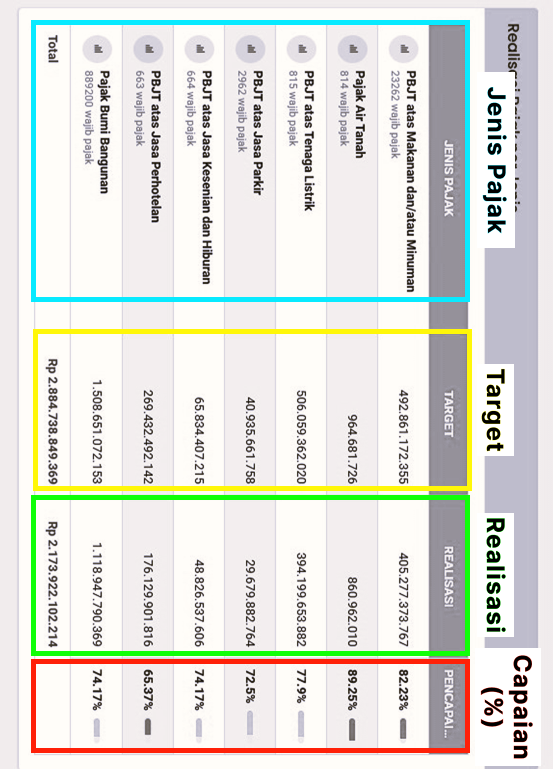
\includegraphics[width=0.76\textwidth]{gambar/wireframe-realisasi-pajak.png}
        \caption{Wireframe Realisasi Pajak}
        \label{fig:wireframe-realisasi-pajak}
    \end{figure}
    \begin{itemize}
        \item \textbf{Fitur Utama:}
            \begin{itemize}
                \item \textbf{Kategorisasi Pajak:} Menampilkan label sektor pajak secara deskriptif (seperti PBJT Makanan, Air Tanah, Tenaga Listrik) untuk mengidentifikasi sumber pendapatan bagi pengguna.
                \item \textbf{Target Finansial:} Menyajikan nominal target penerimaan pajak yang telah ditetapkan dalam periode anggaran tertentu.
                \item \textbf{Realisasi Aktual:} Menampilkan angka riil pendapatan yang telah masuk ke kas daerah berdasarkan transaksi wajib pajak.
                \item \textbf{Indikator Pencapaian:} Berisi perhitungan persentase capaian secara matematis disertai elemen visual berupa \emph{progress bar} berwarna untuk memberikan pemahaman progres secara instan.
            \end{itemize}

        \item \textbf{Analisis Penempatan:}
            \begin{itemize}
                \item \textbf{Penyandingan Horizontal:} Kolom Target dan Realisasi diletakkan berdampingan secara horizontal. Penempatan ini dirancang untuk mempercepat proses kognitif pengguna dalam membandingkan antara sasaran dengan hasil aktual (\emph{plan vs reality}) tanpa perlu memindahkan fokus pandangan terlalu jauh.
                \item \textbf{\emph{Result-Driven Layout}:} Menempatkan kolom Persentase Capaian di posisi paling kanan mengikuti konvensi alur baca manusia dari kiri ke kanan. Hal ini menjadikan kolom tersebut sebagai "titik kesimpulan" atau konklusi dari rincian data finansial yang ada di sebelah kirinya.
                \item \textbf{Efektivitas \emph{Visual Cues}:} Penggunaan \emph{progress bar} berwarnadi akhir kolom memberikan penilaian kinerja secara intuitif. Pengguna dapat langsung mengenali sektor pajak yang memerlukan perhatian khusus melalui visualisasi panjang bar tersebut tanpa harus membaca deretan angka nominal yang panjang, sehingga mendukung prinsip efisiensi operasional sistem \emph{MonPD Reborn}.
            \end{itemize}
    \end{itemize}

\end{itemize}